\documentclass[11pt]{article}
\usepackage[a4paper,margin=1in]{geometry}
\usepackage{booktabs}
\usepackage{amsmath}
\usepackage{xcolor}
\usepackage[hidelinks]{hyperref}
\usepackage{float}
\usepackage{caption}
\usepackage{tikz}
\usepackage{array}
\usepackage{enumitem}
\usepackage{listings}
\usepackage{xspace}
\usetikzlibrary{arrows.meta,calc,positioning,shapes.geometric}

\definecolor{codebg}{RGB}{246,246,246}
\lstset{basicstyle=\ttfamily\small,backgroundcolor=\color{codebg},frame=single,
        rulecolor=\color{black!20},breaklines=true,columns=fullflexible,
        keepspaces=true,showstringspaces=false}
\setlist{itemsep=2pt,topsep=4pt}
\emergencystretch=3em
\newcommand{\code}[1]{\texttt{\detokenize{#1}}}
\newcommand{\st}[1]{\textsc{#1}}
\newcommand{\rupee}{Rs.\,}

\title{\textbf{Strife: A Secure Distributed Payment Gateway}\\[4pt]
\large Two-phase commit over gRPC with durable logs, crash recovery and mutual TLS}
\date{October 2026}

\begin{document}
\sloppy
\maketitle

\begin{abstract}
Strife moves money between accounts held at independent bank servers. A
payment gateway authenticates users and coordinates each transfer with the
two-phase commit (2PC) protocol, so a payment either happens at both banks or
at neither. Every component talks over mutually authenticated TLS, users hold
revocable JWT sessions, and every 2PC vote and decision is written to a SQLite
log before it is acted on, so the system recovers from a crash of the gateway
or of any bank at any point. A chaos experiment that hard-killed components 15
times during 2,747 payments ended with every payment atomic and the total money
unchanged; 39 automated tests cover payments, security and recovery. This
report describes the design, argues its correctness, and presents the
measurements.
\end{abstract}

\section{Project Overview}

Strife simulates the core of a payment processor such as Stripe: clients ask a
gateway to transfer money, and the gateway debits one bank and credits another.
Because the two banks are separate processes with separate storage, the
transfer is a distributed transaction. The system meets the following
requirements:

\begin{itemize}
  \item Bank servers, clients and a payment gateway implemented with gRPC.
  \item Mutual TLS on every connection, with identities checked on both sides.
  \item Authentication, authorization and logging implemented with gRPC
        interceptors.
  \item Idempotent payments: retrying a payment never charges twice.
  \item Offline payments: queued by the client and sent once the gateway is
        reachable again.
  \item Atomic transfers via 2PC with timeouts.
  \item Fault tolerance: durable state at every participant and automatic
        recovery after crashes.
\end{itemize}

\section{System Architecture}

\begin{figure}[H]
\centering
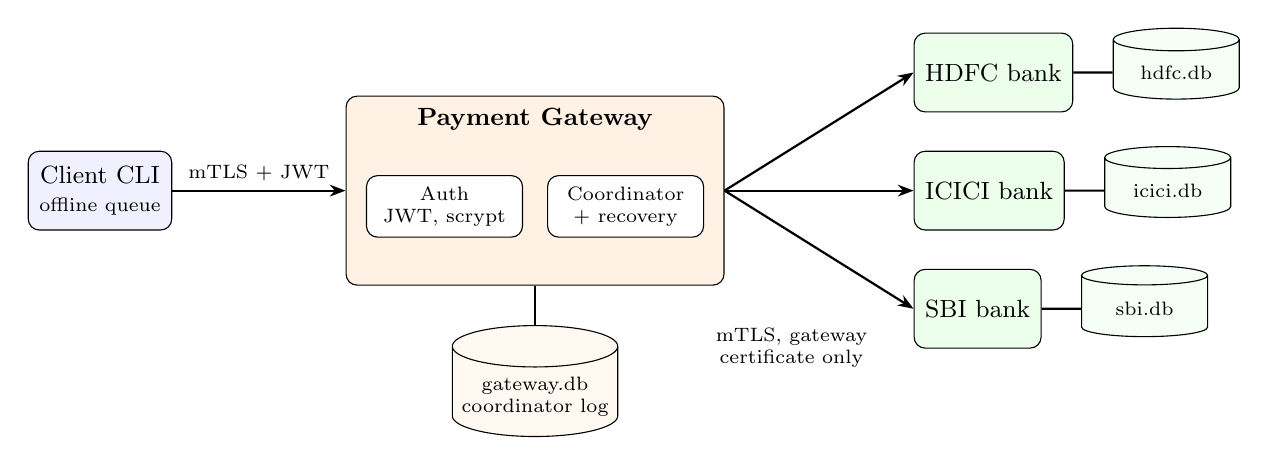
\begin{tikzpicture}[
  box/.style={draw,rounded corners,align=center,minimum height=1.0cm,inner sep=4pt,font=\small},
  db/.style={draw,cylinder,shape border rotate=90,aspect=0.25,align=center,minimum height=0.9cm,minimum width=1.6cm,font=\scriptsize},
  arr/.style={-{Stealth[length=2mm]},thick},
  lbl/.style={font=\scriptsize,fill=white,inner sep=1pt}]
  \node[box,fill=blue!6] (client) {Client CLI\\[-1pt]{\scriptsize offline queue}};
  \node[box,fill=orange!10,right=2.2cm of client,minimum width=4.8cm,minimum height=2.4cm] (gw) {};
  \node[font=\small\bfseries] at ($(gw.north)+(0,-0.3)$) {Payment Gateway};
  \node[box,fill=white,font=\scriptsize,minimum height=0.6cm,text width=1.7cm] at ($(gw.center)+(-1.15,-0.2)$) {Auth\\JWT, scrypt};
  \node[box,fill=white,font=\scriptsize,minimum height=0.6cm,text width=1.7cm] at ($(gw.center)+(1.15,-0.2)$) {Coordinator\\+ recovery};
  \node[db,fill=orange!5,below=0.5cm of gw] (gdb) {gateway.db\\coordinator log};
  \node[box,fill=green!8,right=2.4cm of gw,yshift=1.5cm] (hdfc) {HDFC bank};
  \node[box,fill=green!8,right=2.4cm of gw] (icici) {ICICI bank};
  \node[box,fill=green!8,right=2.4cm of gw,yshift=-1.5cm] (sbi) {SBI bank};
  \foreach \b in {hdfc,icici,sbi} {\node[db,fill=green!4,right=0.5cm of \b] (\b db) {\b.db};
    \draw[thick] (\b) -- (\b db);}
  \draw[arr] (client) -- node[lbl,above=2pt] {mTLS + JWT} (gw);
  \draw[thick] (gw) -- (gdb);
  \draw[arr] (gw.east) -- (hdfc.west);
  \draw[arr] (gw.east) -- (icici.west);
  \draw[arr] (gw.east) -- (sbi.west);
  \node[lbl,align=center] at ($(gw.east)!0.5!(sbi.west)+(-0.35,-1.25)$) {mTLS, gateway\\certificate only};
\end{tikzpicture}
\caption{Components and their durable state. Banks also call
\code{RegisterBank} on the gateway at start-up.}
\end{figure}

\subsection{Payment Gateway (\code{server/payment_gateway.py})}
\begin{itemize}
  \item Central coordinator: validates requests, runs 2PC and answers queries.
  \item Persists payments, the bank directory and revoked tokens in
        \code{gateway.db} (SQLite, WAL mode, \code{fsync} on every commit).
  \item Runs a \emph{recovery worker} that drives in-doubt payments to a final
        state (Section~\ref{sec:recovery}).
  \item gRPC methods: \code{AuthenticateClient}, \code{LogoutClient},
        \code{CheckBalance}, \code{ProcessPayment}, \code{GetPaymentStatus},
        \code{ViewTransactionHistory} and \code{RegisterBank}.
\end{itemize}

\subsection{Bank Servers (\code{server/bank_server.py})}
\begin{itemize}
  \item Each bank is an independent process with its own SQLite ledger
        (\code{<bank>.db}) holding account balances and the 2PC state of every
        transaction it has seen.
  \item Opening balances are loaded from \code{bank_data.json} the first time a
        bank starts; afterwards the ledger is the source of truth.
  \item gRPC methods: \code{GetBalance}, \code{PrepareTransaction},
        \code{CommitTransaction} and \code{AbortTransaction}. Only the gateway's
        certificate may call them.
  \item On start-up the bank registers its host and port with the gateway,
        retrying until the gateway is reachable.
\end{itemize}

\subsection{Client (\code{client/client.py})}
\begin{itemize}
  \item Interactive command-line interface for login, payments, balances,
        history and logout.
  \item Parses rupee amounts exactly (as decimals) and sends integer paise.
  \item Queues payments on disk while the gateway is unreachable and sends them
        automatically when it returns (Section~\ref{sec:offline}).
\end{itemize}

\subsection{Shared modules}
\code{auth.py} (password hashing, login throttling, JWT sessions),
\code{interceptor.py} (authorization, certificate identity, access logging),
\code{tls.py} (mTLS credentials), \code{storage.py} (serialised SQLite
transactions) and \code{config.py} (settings from environment variables).

\subsection{Money representation}
All amounts are 64-bit integers in \emph{paise}. Floating point is never used
for money, so balances cannot drift through rounding (for example
$0.1 + 0.2 \neq 0.3$ in binary floating point).

\section{Authentication \& Security}

\subsection{Mutual TLS and component identity}
A local certificate authority, created by \code{scripts/gen_certs.py}, issues
one certificate per component. Keys are generated locally (or inside Docker and
the test suite) and are never committed to the repository. Both sides of every
connection verify the other's certificate (\code{require_client_auth=True}),
and the certificate's common name (CN) is then used for authorization:

\begin{center}
\begin{tabular}{@{}lll@{}}
\toprule
Component & Certificate CN & May call \\
\midrule
Gateway & \code{gateway} & bank RPCs (the only identity banks accept) \\
Bank & \code{<bank>.bank}, e.g.\ \code{hdfc.bank} & \code{RegisterBank} for \emph{its own} name only \\
Client & \code{client} & user RPCs (plus a valid JWT) \\
\bottomrule
\end{tabular}
\end{center}

Because a bank may only register under the name in its own certificate, a
client or a different bank cannot redirect HDFC's traffic to an address it
controls. Because banks accept only the gateway's certificate, nobody can call
\code{PrepareTransaction} or \code{CommitTransaction} directly to create or
move money. Conversely, user RPCs accept only the client certificate, so a
stolen JWT cannot be used over a bank's or the gateway's certificate.

In the Docker deployment each container mounts a volume holding only its own
key, its certificate and \code{ca.crt}. The CA's private key stays in a volume
that no running service mounts, so compromising one bank container exposes
neither the gateway's key nor the ability to issue new certificates. CI checks
this layout.

\subsection{User authentication}
\begin{itemize}
  \item Passwords are stored as salted scrypt hashes
        ($N=2^{14}, r=8, p=1$) and compared in constant time. A login for an
        unknown user verifies against a dummy hash, so response time does not
        reveal which usernames exist.
  \item Failed logins are rate-limited with two counters stored in
        \code{gateway.db}: five failures in five minutes per
        (username, client address), and twenty per client address across all
        usernames. Either limit blocks further attempts for 60 seconds
        (\code{RESOURCE_EXHAUSTED}). Because the per-user counter includes the
        address, an attacker cannot lock the real user out from elsewhere, and
        the address-wide counter stops password spraying. A restart does not
        reset the counters.
  \item A successful login returns an HS256 JWT with subject, issue time,
        15-minute expiry and a unique id (\code{jti}). The signing key comes
        from \code{PG_JWT_SECRET} and must be at least 32 characters.
  \item Logout revokes the token's \code{jti}. The revocation list is stored in
        \code{gateway.db}, so a revoked token stays invalid across restarts.
\end{itemize}

\subsection{Authorization}
\code{AuthorizationInterceptor} rejects every call without a valid, unexpired,
unrevoked token (except \code{AuthenticateClient} and \code{RegisterBank}) with
\code{UNAUTHENTICATED}. The service then enforces ownership: a user may only
check balances of, and pay from, accounts linked to them
(\code{PERMISSION_DENIED} otherwise), and may only see the status of payments
they sent or received.

\subsection{Input validation}
The server validates every payment independently of the client:
\begin{itemize}
  \item the amount must be between 1 paisa and \rupee10,00,000 (banks
        additionally refuse non-positive amounts);
  \item the receiver account must exist (\code{NOT_FOUND});
  \item sender and receiver accounts must differ;
  \item the transaction id must be 1--64 characters from \code{[A-Za-z0-9_-]}.
\end{itemize}
Each failure returns a specific gRPC status code (\code{INVALID_ARGUMENT},
\code{NOT_FOUND}, \code{PERMISSION_DENIED}) rather than a generic error.

\section{Transaction Processing (2PC)}
\label{sec:2pc}

\begin{figure}[H]
\centering
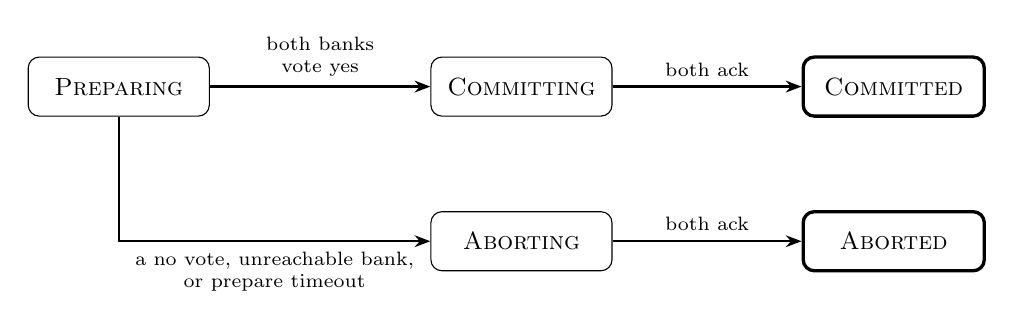
\begin{tikzpicture}[
  st/.style={draw,rounded corners,minimum width=2.3cm,minimum height=0.75cm,font=\small\scshape},
  fin/.style={st,very thick},
  arr/.style={-{Stealth[length=2mm]},thick},
  lbl/.style={font=\scriptsize,align=center}]
  \node[st] (p) {Preparing};
  \node[st,right=2.8cm of p] (c) {Committing};
  \node[fin,right=2.4cm of c] (cd) {Committed};
  \node[st,below=1.2cm of c] (a) {Aborting};
  \node[fin,right=2.4cm of a] (ad) {Aborted};
  \draw[arr] (p) -- node[lbl,above] {both banks\\vote yes} (c);
  \draw[arr] (c) -- node[lbl,above] {both ack} (cd);
  \draw[arr] (p) |- node[lbl,pos=0.75,below] {a no vote, unreachable bank,\\or prepare timeout} (a);
  \draw[arr] (a) -- node[lbl,above] {both ack} (ad);
\end{tikzpicture}
\caption{Payment states in the coordinator log. Every transition is a
compare-and-set on the stored status.}
\end{figure}

\subsection{Phase 0: log the payment}
After validation the gateway inserts the payment into \code{gateway.db} with
status \st{Preparing}. The client-generated transaction id is the primary key.

\subsection{Phase 1: prepare}
The gateway asks, in parallel, the sender's bank to prepare a \st{Debit} and
the receiver's bank to prepare a \st{Credit}. Each bank votes inside one serialised SQLite
transaction (\code{BEGIN IMMEDIATE}):
\begin{itemize}
  \item \textbf{Debit:} vote yes only if
        $\text{balance} - \text{reserved} \ge \text{amount}$, where
        \emph{reserved} is the sum of the account's other prepared debits; the
        vote itself records a reservation of \emph{amount}.
  \item \textbf{Credit:} vote yes if the account exists.
\end{itemize}
The vote is written to disk before the reply is sent. A repeated prepare for
the same transaction returns the original vote.

\subsection{Decision}
If both banks vote yes, the gateway changes the status from \st{Preparing} to
\st{Committing}; otherwise to \st{Aborting}, storing the reason (for example
``Insufficient funds''). The decision is durable \emph{before} any bank is told
about it.

\subsection{Phase 2: commit or abort}
The gateway sends the decision to both banks. Both operations are idempotent:
\begin{itemize}
  \item \textbf{Commit} applies the debit or credit and marks the entry
        committed; repeating it is a no-op.
  \item \textbf{Abort} releases the reservation. An abort for a transaction the
        bank never saw writes a \emph{tombstone}, so a delayed prepare that
        arrives afterwards is refused.
\end{itemize}
When both banks acknowledge, the status becomes \st{Committed} or
\st{Aborted}. If a bank cannot be reached, the payment stays in
\st{Committing}/\st{Aborting} and the recovery worker retries. A client whose
payment is \st{Committing} is told it succeeded: the decision is final and will
be applied.

\subsection{Timeouts and recovery}
\label{sec:recovery}
Every gateway-to-bank call has a 3-second deadline. The recovery worker runs
every 2 seconds, and immediately when the gateway starts:
\begin{itemize}
  \item \st{Committing}/\st{Aborting}: resend the decision to both banks until
        both acknowledge.
  \item \st{Preparing} for longer than 30 seconds: the coordinator crashed or
        stalled before deciding. No commit decision exists, so the payment is
        moved to \st{Aborting} (\emph{presumed abort}) and the reservations are
        released.
\end{itemize}
Both the request thread and the recovery worker change state only by
compare-and-set, so exactly one decision is ever recorded, even if they race.

\section{Idempotent Payment Processing}

\subsection{Implementation}
The client generates a random 128-bit transaction id for each payment and
reuses it for every retry, including retries from the offline queue. The id is
the primary key of the coordinator log:
\begin{itemize}
  \item a new id starts a new payment;
  \item an id seen before \emph{with the same user and parameters} returns the
        stored outcome (\st{Committed}, \st{Aborted}, or ``in progress'')
        without touching the banks;
  \item an id seen before with a different user or different parameters is
        rejected with \code{ALREADY_EXISTS}, so ids cannot be hijacked.
\end{itemize}

\subsection{Correctness arguments}
We assume the gateway and every bank eventually restart after a crash with
their disks intact, and that the network eventually delivers messages between
live processes.

\paragraph{Exactly-once (no double charge).}
Inserting a payment and checking for an existing id happen in one SQLite
transaction, and the id is a primary key, so at most one payment record exists
per id. The banks key their ledger entries on (transaction id, operation), so
even a prepare or commit retried by the gateway affects each account at most
once. Therefore a payment is applied at most once however often the client
retries.

\paragraph{Atomicity.}
The decision is a single compare-and-set from \st{Preparing}, so it is
recorded exactly once and never changes. A bank applies a commit only for an
entry it prepared, and only when the gateway sends \st{Commit}, which it does
only after logging \st{Committing}; a bank releases a reservation only on
\st{Abort}. Hence the two banks can never apply different outcomes. Because
votes and decisions are durable, a crash of either side loses neither; and
because phase 2 is idempotent and retried until acknowledged, both banks
eventually apply the logged decision.

\paragraph{No overdraft or double spend.}
Each bank maintains the invariant
$\text{balance} - \text{reserved} \ge 0$ for every account. Prepare checks it
and adds the reservation in one serialised transaction, so two concurrent debits
cannot both pass the check against the same funds. A committed debit subtracts
an amount that was already reserved, so the balance never goes negative. A
database \code{CHECK} constraint enforces this as well.

\paragraph{Conservation of money.}
Every committed payment applies a debit and a credit of the same amount, and by
atomicity they are applied together or not at all. The total money across all
banks is therefore constant. The chaos experiment
(Section~\ref{sec:chaos}) checks exactly this.

\paragraph{Liveness and its limit.}
Under the assumptions above, every payment reaches \st{Committed} or
\st{Aborted}. 2PC is, however, a \emph{blocking} protocol: while the gateway is
down, a bank that voted yes must keep its reservation, because it cannot know
the decision. The funds are safe but unavailable until the gateway returns.

\section{Offline Payments \& Retry Mechanism}
\label{sec:offline}

\subsection{Client-side queuing}
\begin{itemize}
  \item Each RPC is retried up to three times while the gateway reports
        \code{UNAVAILABLE} or the deadline expires.
  \item If the gateway is still unreachable, the payment, with its transaction
        id, is appended to \code{offline_payments.json} and survives client
        restarts.
\end{itemize}

\subsection{Automatic resending}
A background thread checks the channel's connectivity every 10 seconds (without
sending fake requests) and, once the gateway is reachable and the user is logged
in, resends queued payments. A payment leaves the queue once the gateway gives
any final answer: completed, aborted for insufficient funds, or rejected as
invalid. Because the transaction id is unchanged, a payment that had reached the
gateway before the connection dropped is not applied a second time.

\subsection{Failure handling}
\begin{center}
\begin{tabular}{@{}p{4.5cm}p{10cm}@{}}
\toprule
Failure & Behaviour \\
\midrule
Gateway down & Client queues the payment; it is sent once the gateway returns. \\
Response lost after the gateway processed it & Resend returns the stored outcome; no second charge. \\
Bank down during prepare & Payment aborts; the other bank's reservation is released; the unreachable bank's abort is delivered when it returns. \\
Bank down during commit & Payment stays \st{Committing}; recovery commits when the bank returns (its yes vote is on disk). \\
Gateway crash after the decision & On restart, recovery delivers the logged decision. \\
Gateway crash before the decision & After the prepare timeout, presumed abort releases the reservations. \\
Delayed prepare after an abort & Refused because of the abort tombstone. \\
\bottomrule
\end{tabular}
\end{center}

\section{Logging \& Monitoring}
\begin{itemize}
  \item \code{LoggingInterceptor} records every RPC with its method, final
        status code, latency and peer address.
  \item \code{AuthorizationInterceptor} and \code{PeerIdentityInterceptor} log
        each rejected call and its reason.
  \item The coordinator logs each payment's progress (prepare votes, decision,
        phase-2 retries, recoveries). Banks log every vote, commit and abort.
  \item The authoritative history is the coordinator log in \code{gateway.db},
        which \code{ViewTransactionHistory} and \code{GetPaymentStatus} query.
        Users see the sender's account number only on their own outgoing
        payments.
\end{itemize}

\section{Evaluation}

\subsection{Automated tests}
39 pytest tests start a gateway and three banks in-process on free ports:
\begin{itemize}
  \item \textbf{Payments (7):} cross-bank transfer; insufficient funds;
        server-side rejection of zero, negative and oversized amounts; specific
        error codes; idempotent retries; a double-spend attempt with 40
        concurrent \rupee100 payments against a \rupee1,500 balance (exactly 15
        succeed); 120 random concurrent transfers that must conserve money.
  \item \textbf{Security (13):} missing, forged, expired and revoked tokens;
        revocation surviving a restart; login lock-out scoped to the client
        address and surviving a restart; password spraying; access to another
        user's account; bank impersonation; non-client certificates on user
        RPCs; non-gateway callers at a bank; the per-component key layout.
  \item \textbf{Recovery (7):} receiver commit failure; bank down during
        prepare; gateway crash after the decision; gateway crash before the
        decision; bank crash after voting yes; late prepare after abort;
        malformed operation.
  \item \textbf{Client (12):} exact rupee parsing, and an offline payment sent
        exactly once after the gateway returns.
\end{itemize}

\subsection{Chaos experiment}
\label{sec:chaos}
\code{scripts/chaos_demo.py} runs the gateway and the three banks as separate
operating-system processes. Eight client threads send random payments while,
every 1--3 seconds, a random component is hard-killed
(\code{SIGKILL}/\code{TerminateProcess}, so no clean-up code runs) and
restarted. After the load stops and recovery settles, an audit compares the
coordinator log with every bank ledger. Result of a 40-second run:

\begin{center}
\begin{tabular}{@{}lr@{}}
\toprule
Measure & Value \\
\midrule
Components killed (gateway / HDFC / ICICI / SBI) & 15 (4 / 5 / 2 / 4) \\
Payments logged & 2,747 \\
\quad committed / aborted & 2,264 / 483 \\
Client calls that failed with \code{UNAVAILABLE} & 32 \\
In-doubt payments settled by the recovery worker & 158 (117 committed, 41 aborted) \\
\quad of which presumed aborted after a gateway crash & 10 \\
Payments left in doubt, or reservations left held & 0 \\
Payments where the two banks disagree & 0 \\
Money before / after & \rupee23,000.00 / \rupee23,000.00 \\
\bottomrule
\end{tabular}
\end{center}

The aborts combine insufficient-funds outcomes (the workload draws random
amounts against small balances) with payments that a kill interrupted before a
commit decision.

\subsection{Throughput and latency}
\code{scripts/benchmark.py} runs the same multi-process deployment (mTLS on
every hop) and measures completed payments per second at several client
concurrencies (8 seconds per level, Windows laptop). Each payment performs four
gateway-to-bank calls and seven durable writes: three at the gateway and two at
each bank.

\begin{figure}[H]
\centering
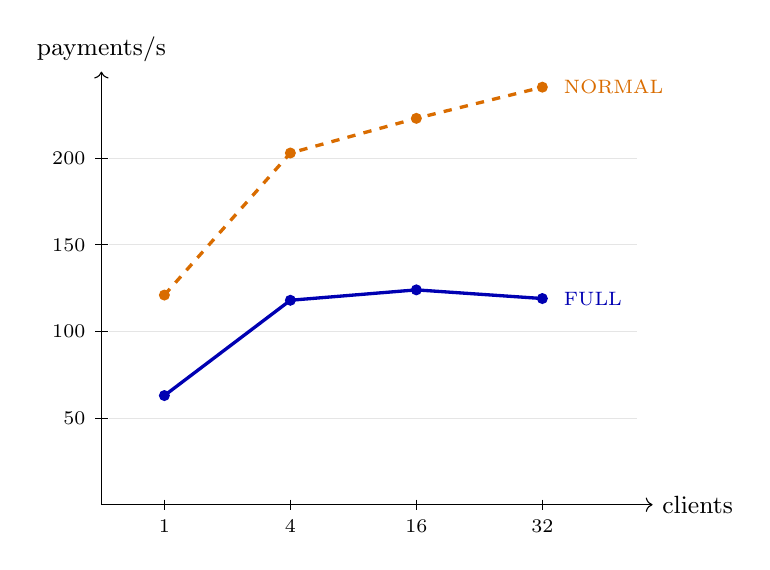
\begin{tikzpicture}[x=1.0cm,y=0.022cm]
  \draw[->] (0,0) -- (7.0,0) node[right,font=\small] {clients};
  \draw[->] (0,0) -- (0,250) node[above,font=\small] {payments/s};
  \foreach \y in {50,100,150,200} {\draw (0.08,\y) -- (-0.08,\y) node[left,font=\scriptsize] {\y};
    \draw[black!10] (0.1,\y) -- (6.8,\y);}
  \foreach \x/\l in {0.8/1,2.4/4,4.0/16,5.6/32} {\draw (\x,3) -- (\x,-3) node[below,font=\scriptsize] {\l};}
  \draw[very thick,blue!70!black] (0.8,63) -- (2.4,118) -- (4.0,124) -- (5.6,119);
  \foreach \x/\y in {0.8/63,2.4/118,4.0/124,5.6/119} {\fill[blue!70!black] (\x,\y) circle (2pt);}
  \draw[very thick,orange!85!black,dashed] (0.8,121) -- (2.4,203) -- (4.0,223) -- (5.6,241);
  \foreach \x/\y in {0.8/121,2.4/203,4.0/223,5.6/241} {\fill[orange!85!black] (\x,\y) circle (2pt);}
  \node[font=\scriptsize,blue!70!black,anchor=west] at (5.75,119) {FULL};
  \node[font=\scriptsize,orange!85!black,anchor=west] at (5.75,241) {NORMAL};
\end{tikzpicture}
\caption{Throughput with SQLite \code{synchronous=FULL} (fsync on every commit,
the default) and \code{NORMAL}.}
\end{figure}

\begin{center}
\begin{tabular}{@{}rrrrr@{}}
\toprule
& \multicolumn{2}{c}{\code{FULL} (default)} & \multicolumn{2}{c}{\code{NORMAL}} \\
\cmidrule(lr){2-3}\cmidrule(lr){4-5}
Clients & TPS & p50 / p99 (ms) & TPS & p50 / p99 (ms) \\
\midrule
1  & 63  & 15 / 28   & 121 & 8 / 15 \\
4  & 118 & 33 / 48   & 203 & 18 / 44 \\
16 & 124 & 128 / 172 & 223 & 66 / 126 \\
32 & 119 & 247 / 636 & 241 & 129 / 206 \\
\bottomrule
\end{tabular}
\end{center}

\paragraph{Discussion.}
With full durability, throughput is limited by disk flushes, not by gRPC or
TLS. Every commit waits for an fsync, and each process issues its writes one at
a time, so beyond about four clients extra clients mostly add queueing delay.
Relaxing to \code{NORMAL} roughly doubles throughput. In WAL mode that setting
still survives process crashes, but it may lose the last commits on an
operating-system crash or power loss. \code{FULL} results also vary by up to
2--3$\times$ between runs on this laptop, because flush latency is noisy. The
usual way to keep full durability at higher throughput is \emph{group commit}:
one fsync shared by the writes of many concurrent payments.

\paragraph{Parallel prepare.}
The gateway asks both banks to prepare at the same time. An A/B comparison
alternated three runs each of sequential and parallel prepare under
\code{NORMAL}. Parallel prepare cut single-client median latency from 10.2\,ms
to 8.1\,ms and raised single-client throughput from 92 to 110 payments/s. At
4--16 clients the two were within run-to-run noise: there, throughput is
limited by serialised database writes rather than by the extra round trip.
Under \code{FULL} the fsync noise exceeded the difference.

\section{Assumptions}
\begin{enumerate}
  \item Users are predefined in \code{users.json} (with hashed passwords); there
        is no self-registration. New users are added with
        \code{scripts/hash_password.py}.
  \item A user has at most one account per bank, so a bank name identifies the
        account unambiguously.
  \item Every component has a certificate issued by the deployment's CA before
        it starts.
  \item Banks and clients know the gateway's address
        (\code{PG_GATEWAY_ADDRESS}); banks tell the gateway their own address
        when they register.
  \item Crashed processes eventually restart with their disks intact.
\end{enumerate}

\section{Deployment}
\code{docker compose up} runs a one-shot job that creates the CA and writes
each component's credentials into its own volume, then starts the gateway and
the three banks, each with its own credentials and data volumes. The client
runs with \code{docker compose run client}. GitHub Actions runs the test suite,
the chaos experiment, a check that the generated protobuf code is up to date,
and a Docker Compose smoke test that also verifies each container holds only
its own key.

\section{Limitations \& Future Enhancements}
\begin{itemize}
  \item \textbf{Coordinator availability.} The gateway is a single coordinator,
        and 2PC blocks while it is down. Replicating the coordinator log with a
        consensus protocol (Raft or Paxos), as Spanner does, would let another
        replica finish in-doubt payments.
  \item \textbf{Storage.} SQLite with one connection per process serialises
        writes. PostgreSQL with group commit would raise throughput while
        keeping full durability.
  \item \textbf{Identity.} Users come from a JSON file, and tokens are signed
        with one shared HS256 key. A production system would use a user
        database and asymmetric signing keys (RS256 or EdDSA) with rotation.
  \item \textbf{Operations.} Metrics such as Prometheus counters for payment
        outcomes and recovery backlog, and an admin view of in-doubt payments.
\end{itemize}

\end{document}
